\documentclass[20pt, a0paper, landscape, margin=15mm, innermargin=20mm, blockverticalspace=12mm]{tikzposter}
\usepackage[utf8]{inputenc}
\usepackage{amsmath,amssymb}
\usepackage{graphicx}
\usepackage{booktabs}
\usepackage{xcolor}
\usepackage{enumitem}

\definecolor{DarkBlue}{HTML}{1B2A4A}
\definecolor{AccentOrange}{HTML}{E8752A}
\definecolor{AccentTeal}{HTML}{0F9B8E}
\definecolor{AlertRed}{HTML}{C0392B}

\colorlet{blocktitlebgcolor}{DarkBlue}
\colorlet{blocktitlefgcolor}{white}
\colorlet{blockbodybgcolor}{white}
\colorlet{blockbodyfgcolor}{black}

\usetheme{Default}
\usetitlestyle{Default}
\useblockstyle{Minimal}

\title{\shortstack{\textbf{How Stable Are Regression Conclusions Across Subpopulations?}\\[2mm] \large A Finite-Sample Empirical Study}}
\titlegraphic{\includegraphics[height=2.5cm]{AUB_Main_Horizontal_RGB.pdf}}
\author{[Authors] -- Department of Statistics -- July 2026}

\begin{document}
\maketitle

\begin{columns}

%% ═══════════════════════════════════════ LEFT COLUMN (0.30)
\column{0.30}

\block{The Problem}{
  You fit a regression on the full dataset. $R^2$ is fine, p-values are small.
  A reviewer asks: \textit{``Does this hold for each subgroup?''}
  \begin{center}
    \textbf{You check. It doesn't. Now what?}
  \end{center}
}

\block{Simpson's Paradox}{
  \begin{center}
    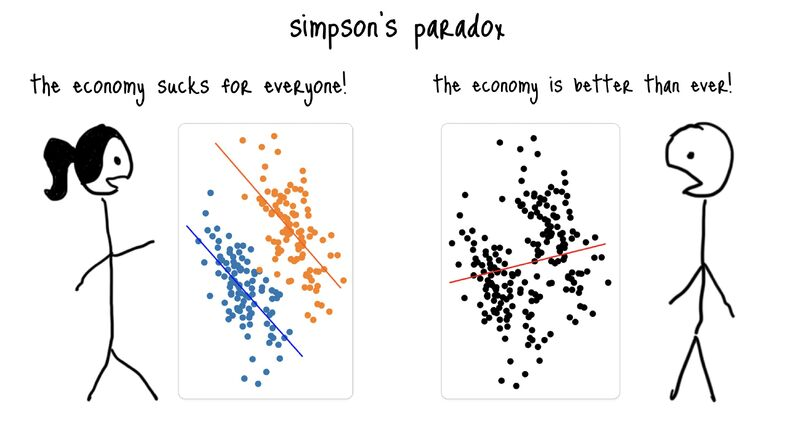
\includegraphics[width=0.85\linewidth]{simpson.jpg}
  \end{center}
  Within each group the trend is positive. Pooled, it reverses. The pooled regression hides subgroup structure.
}

\block{``It's an Artifact''}{
  \begin{center}
    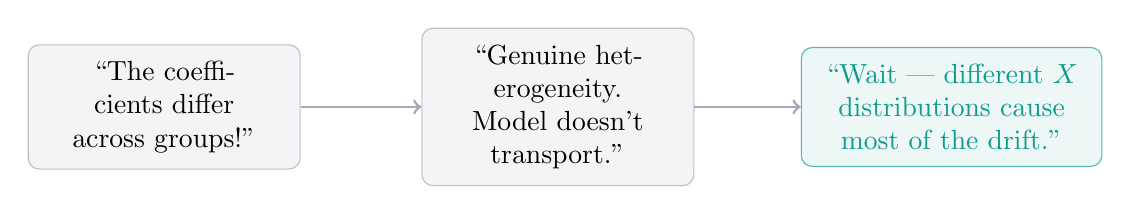
\begin{tikzpicture}[every node/.style={align=center}]
      \node[draw=DarkBlue!30, fill=DarkBlue!5, rounded corners=4pt,
            inner sep=6pt, text width=0.25\linewidth] (A) at (0,0) {
            ``The coefficients differ\\across groups!''
          };
      \node[draw=DarkBlue!30, fill=DarkBlue!5, rounded corners=4pt,
            inner sep=6pt, text width=0.25\linewidth] (B) at (5,0) {
            ``Genuine heterogeneity.\\Model doesn't transport.''
          };
      \node[draw=AccentTeal!70, fill=AccentTeal!8, rounded corners=4pt,
            inner sep=6pt, text width=0.28\linewidth] (C) at (10,0) {
            \color{AccentTeal}``Wait --- different $X$\\ distributions cause\\most of the drift.''
          };
      \draw[->, DarkBlue!40, line width=1pt] (A.east) -- (B.west);
      \draw[->, DarkBlue!40, line width=1pt] (B.east) -- (C.west);
    \end{tikzpicture}
  \end{center}
  Coefficient differences come from \textbf{two sources}: genuine heterogeneity and mechanical artifacts from covariate distribution differences. Standard practice conflates them.
}


%% ═══════════════════════════════════════ CENTER COLUMN (0.40)
\column{0.40}

\block{Real-Data Evidence: NHANES Blood Pressure}{
  \textbf{Data:} NHANES 2017--2018 ($n=9{,}254$), systolic BP response, age-decade subgroups.
  Predictors: BMI, waist circumference, total cholesterol, HDL.

  \begin{center}
    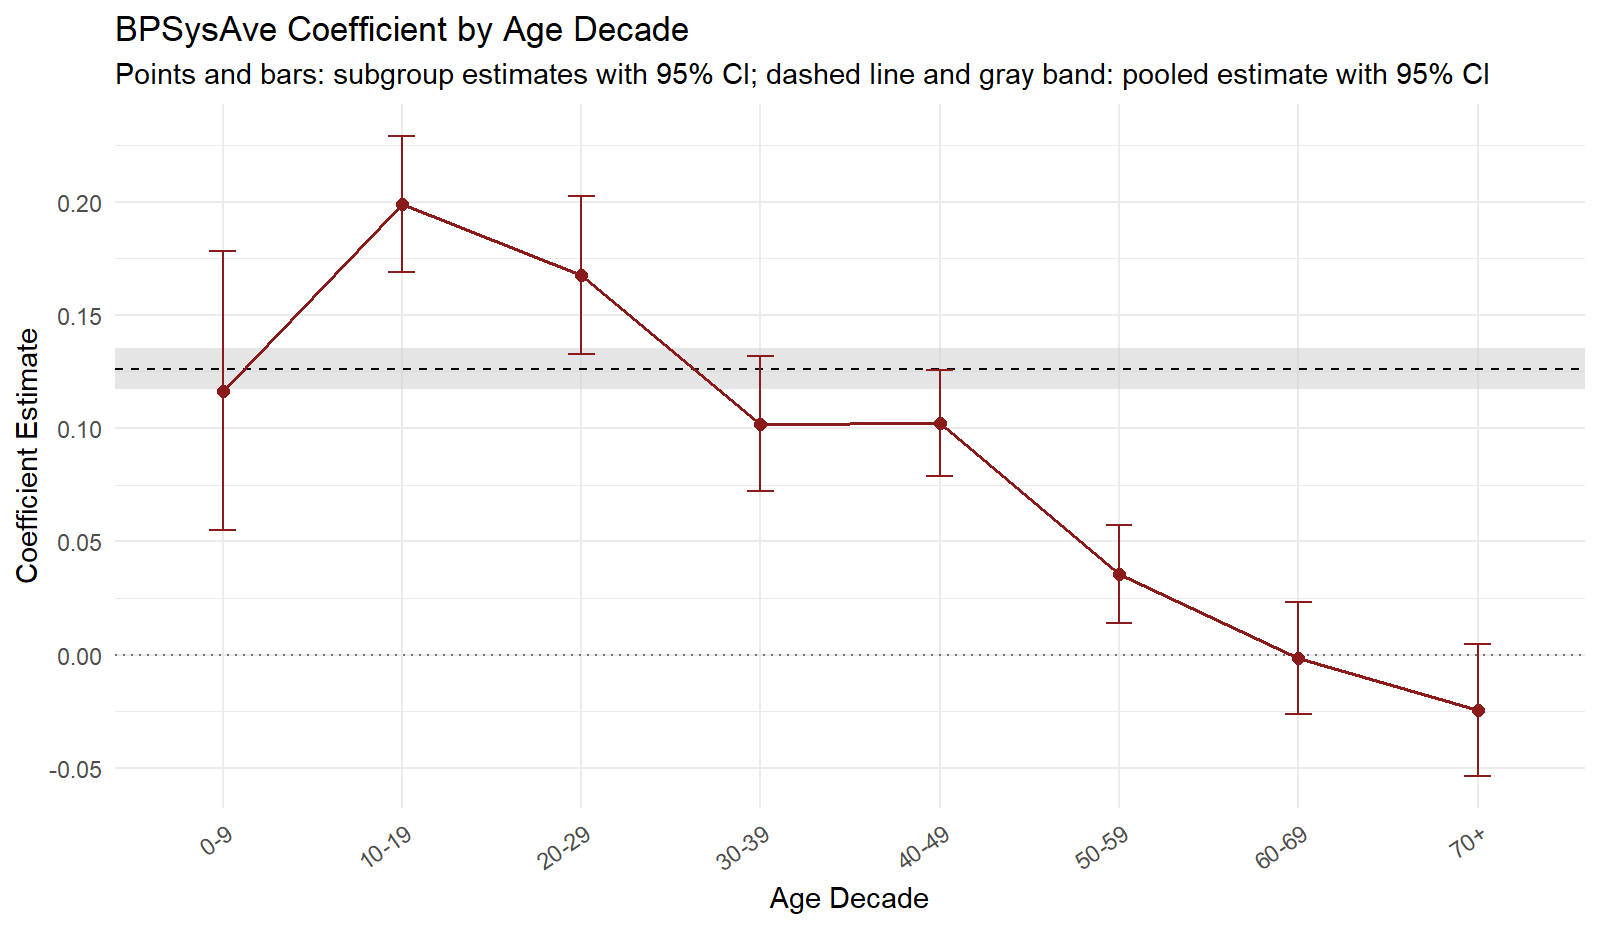
\includegraphics[width=0.85\linewidth]{../results/nhanes_age_decade/bpsys_coef_by_age_decade_ci.png}
  \end{center}

  \begin{tabular}{@{}lrr@{}}
    \toprule
    \textbf{Metric} & \textbf{Value} \\
    \midrule
    SSR (all predictors)     & 0.57 \\
    Max standardized drift   & 32.07 (BPSysAve) \\
    Context-norm.\ drift     & 7.49 (BPSysAve) \\
    Avg.\ CSS (pairwise)     & 0.28 \\
    \bottomrule
  \end{tabular}

  \textbf{Key finding:} Waist circumference's effect on BP \textit{reverses sign} in older groups. Drift 32$\to$7.5 after context normalization, confirming genuine heterogeneity.
}

\block{Five Stability Metrics}{
  \begin{tabular}{@{}p{0.15\linewidth} p{0.38\linewidth} p{0.40\linewidth}@{}}
    \toprule
    \textbf{Metric} & \textbf{Definition} & \textbf{What it captures} \\
    \midrule
    SSR
    & $\mathrm{SSR}_j = \frac{1}{M}\sum \mathbf{1}(\mathrm{sgn}\,\hat\beta_{j,a}=\mathrm{sgn}\,\hat\beta_{j,b})$
    & Do conclusions ($+$/$-$) reverse across groups? \\[6pt]

    Standardized drift
    & $D_j^\star = \frac{\max_g|\hat\beta_{j,g} - \hat\beta_{j,\text{pooled}}|}{\widehat{\text{SE}}(\hat\beta_{j,\text{pooled}})}$
    & How far do subgroup coefficients move from pooled, in SE units? \\[6pt]

    Context-norm.\ drift
    & $\widetilde{D}_j = \dfrac{D_j^\star}{1 + M_j}$,\newline
      $M_j = \frac{1}{\binom{G}{2}}\sum_{a<b}\frac{|\bar{x}_{j,a}-\bar{x}_{j,b}|}{s_{j,\text{pooled}}}$
    & Drift after accounting for covariate distribution differences. \\[6pt]

    TPG
    & $\mathrm{TPG}_{a\to b} = \mathrm{RMSE}_{\text{pooled}\to b} - \mathrm{RMSE}_{b\to b}$
    & Prediction loss when a model travels across groups. \\[6pt]

    CSS
    & $\mathrm{CSS}_{a,b} = \frac{1}{p}\sum_{j}\frac{|\bar{x}_{j,a} - \bar{x}_{j,b}|}{s_{j,\text{pooled}}}$
    & How different are $X$ distributions between groups? \\
    \bottomrule
  \end{tabular}
}

\block{Key Decomposition: Why Context Drift $<$ Raw Drift}{
  Even with identical $\beta$, different $X$ distributions inflate drift:
  \[
    \hat\beta^{(g)} - \hat\beta^{(\text{pooled})} = (X_g'X_g)^{-1}X_g'\varepsilon_g - (X'X)^{-1}X'\varepsilon
  \]
  \begin{center}
    \colorbox{DarkBlue!5}{$D_j^\star \;=\; \widetilde{D}_j \;\times\; (1 + M_j)$}\\[2pt]
    {\footnotesize Total = Genuine $\times$ Mechanical}
  \end{center}
  3 regimes: $M_j\approx 0 \Rightarrow$ all drift real; large $M_j$ + small $\widetilde{D}_j \Rightarrow$ artifact; both large $\Rightarrow$ genuine heterogeneity.
}


%% ═══════════════════════════════════════ RIGHT COLUMN (0.30)
\column{0.30}

\block{Four Models (nested)}{
  M1: pooled $Y = \beta_0 + X^\top\beta + \varepsilon$\\
  M2: add group intercept $\gamma G$\\
  M3: add interactions $X^\top\delta G$\\
  M4: fully separate model per group
}

\block{Simulation Grid (Scenario 1)}{
  \textbf{140 settings:} $G \in \{3,5,10,20,40\}$, $n \in \{100,\dots,30000\}$,
  4 imbalance patterns (balanced, mild, strong, Dirichlet-random). 200 reps each.

  \begin{center}
    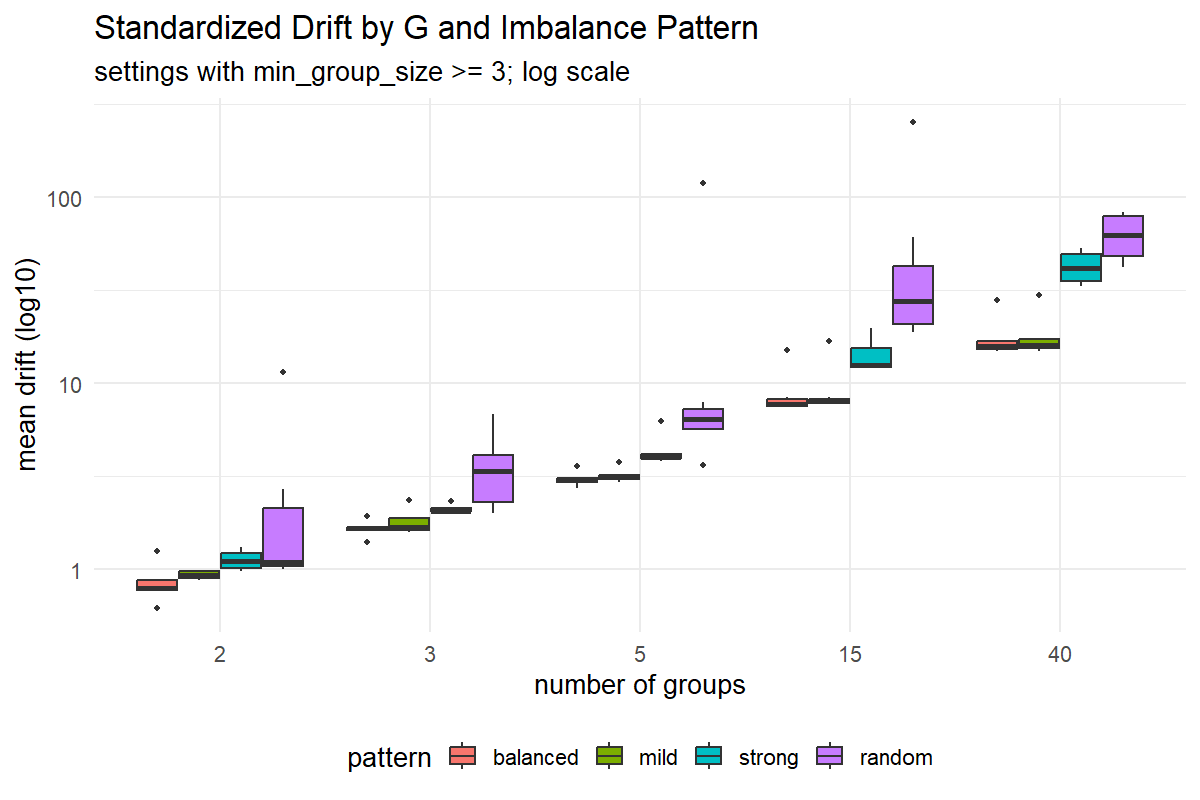
\includegraphics[width=0.47\linewidth]{../results/simulation/drift_by_G_and_pattern.png}\hfill
    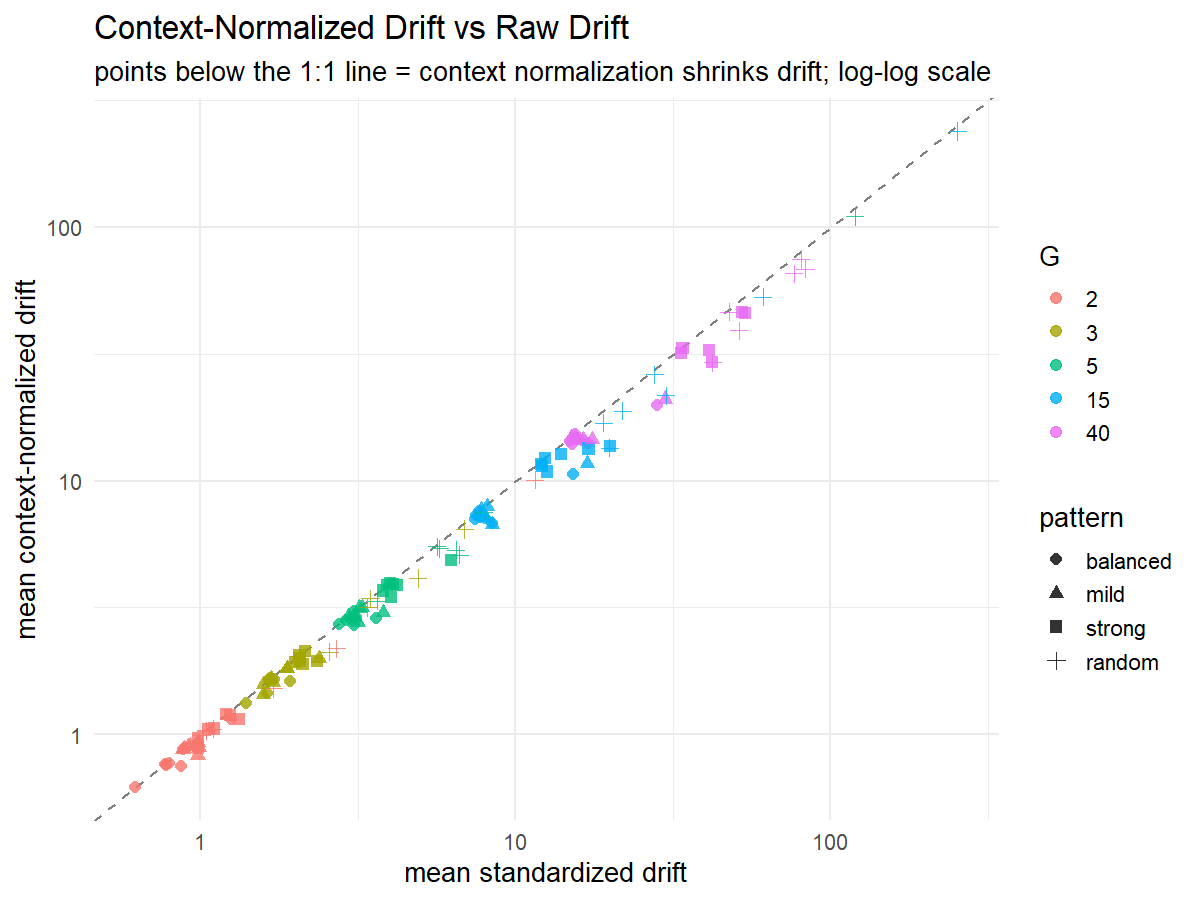
\includegraphics[width=0.47\linewidth]{../results/simulation/context_vs_raw_drift.png}
  \end{center}
  Drift grows with $G$ and imbalance (left). Context normalization shrinks drift (right).
}

\block{What Drives Instability?}{
  \begin{itemize}[leftmargin=*, itemsep=2pt]
    \item Drift driven by $G$ and per-group $n$, not total $N$.
    \item Strong/random imbalance amplifies drift 2--4$\times$ over balanced.
    \item SSR = 1.0 throughout (Scenario 1: identical $\beta$, no sign flips).
    \item Context normalization reduces drift; shrinkage $\propto$ CSS.
  \end{itemize}
}

\block{Future Work}{
  Same analysis for Scenarios 2--4, then:
  \begin{enumerate}[leftmargin=*, itemsep=2pt]
    \item Introduce \textbf{collinearity} across predictors
    \item Scale to \textbf{higher dimensions} (more predictors)
    \item Test \textbf{different regression models} beyond OLS
  \end{enumerate}
}

\block{References}{
  \scriptsize
  Berk et al.\ (2019); Tsoi et al.\ (2026); Bertsimas \& Paskov (2020);
  Liu et al.\ (2020); Watson \& Engle (1985); Garbade (1977); Buja et al.\ (2006).
  \hfill {\tiny \texttt{github.com/Nadjoubiii/Regression-conclusion-stability-paper}}
}

\end{columns}
\end{document}
